\section{Facial Expression Recognition}
The development of the Pookie AI-driven robot incorporates a crucial element: detecting and interpreting user emotions, particularly stress and anxiety, using Facial Emotion Recognition (FER). This section outlines the current progress, challenges, and future approaches for designing the emotion detection system, including relevant datasets, models, and methodologies.
\subsection{As-is Behavior}
Initially, the facial expression recognition model for this project was expected to use a model fine tuning approach over a Chinese Faces Dataset, as it provides the most symmetric resemblance to a Thai dataset, which is difficult to obtain. The foundation model used was a VGGNet architecture (Figure 2), a multi layer convolutional neural network often used for feature extraction and classification tasks, with a notable variety of emotion detection models stemming from it. 

\begin{figure}[ht]
    \centering
    \captionsetup{justification=centering}
    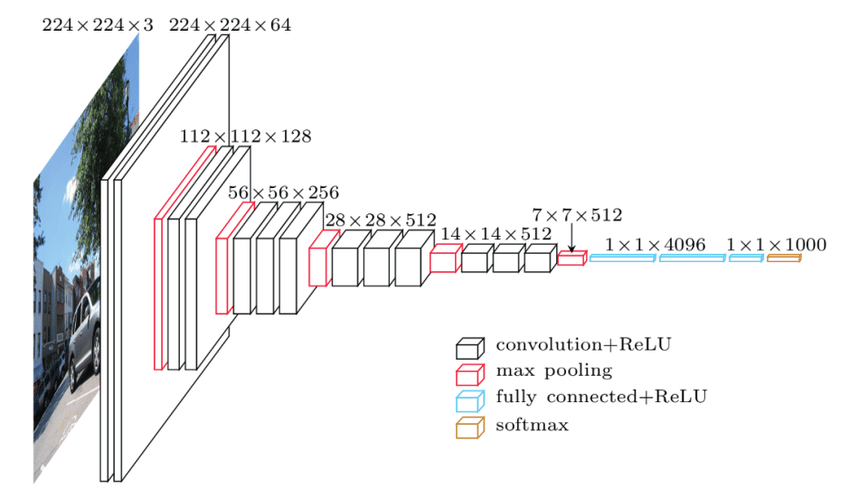
\includegraphics[width=0.9\textwidth]{vggnet.png}
    \caption{VGGNet Architecture}
    \label{fig:vggnet}
\end{figure}

For our approach, we took a pre-trained model for emotion recognition using VGGNet architecture, then fine tuned the inference layers on a Chinese dataset in order to get more accurate representation for Thai faces. The other layers were frozen, and served as foundation parameters for transfer learning. After multiple versions of the model, however, it could be seen that this approach did not yield great results. As shown in Figure 3, the model yielded results far worse than simple guessing, most likely due to inappropriate usage of transfer learning on an already imperfect model. 

\begin{figure}[ht]
    \centering
    \captionsetup{justification=centering}
    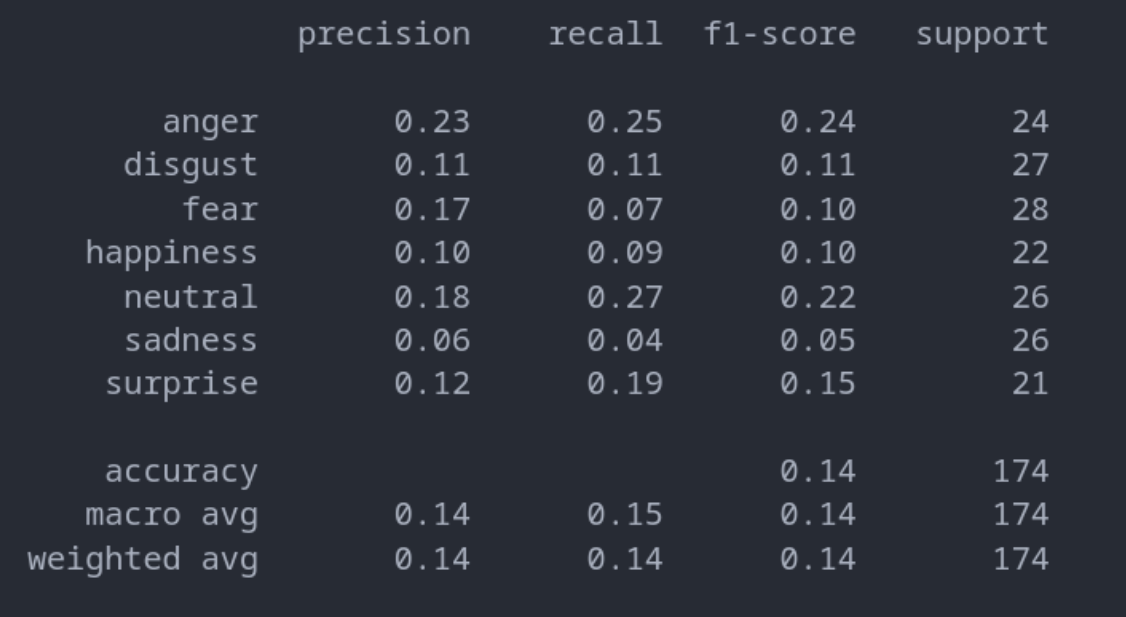
\includegraphics[width=0.67\textwidth]{finetune.png}
    \caption{Fine Tuning Results}
    \label{fig:finetune}
\end{figure}

\newpage
\subsection{Refined Approach}
After consultation with our advisor, we were recommended to revise our research on facial emotion recognition, where some of the assumptions and approaches we had initially proven to be wrong. Initially, the fine tuning approach was meant to familiarize the pre-trained VGGNet with a new dataset that could be ignored or underrepresented. However, the use case of fine tuning and transfer learning requires careful consideration. Thus, instead of fine tuning the model over the Chinese dataset, we instead included the Chinese dataset in the training and validation sets, where instead of using pre-trained weights, we trained an emotion detection model following the VGGNet architecture from scratch, which yielded significantly better results, as shown in Figure 4.

\begin{figure}[ht]
    \centering
    \captionsetup{justification=centering}
    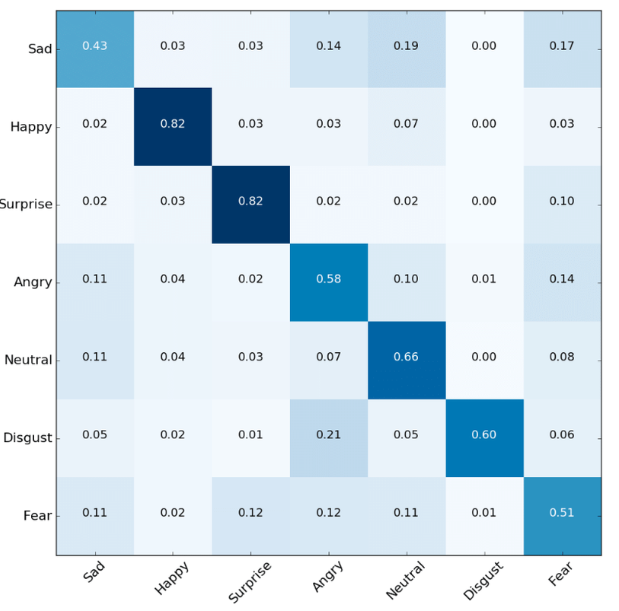
\includegraphics[width=0.8\textwidth]{refined.png}
    \caption{Refined Approach Results}
    \label{fig:refined}
\end{figure}

As seen in the results, the model is great at distinguishing between positive emotions such as happiness or surprise, but it is quite lacking in negative emotions. However, given the scope of the project, where positive and neutral are associated with specific outputs, and negative emotions are all classified as stress, then the model is generally enough to use as a minimum viable product for the rest of the semester.

\subsection{Next Steps}
The next steps for facial emotion recognition is to integrate this model with the SER server to have a common ground for communication and output. Although the model is not perfect, it is viable enough to be used for a prototype for the rest of the semester, where other parts will be prioritized from now on.
